
%(BEGIN_QUESTION)
% Copyright 2012, Tony R. Kuphaldt, released under the Creative Commons Attribution License (v 1.0)
% This means you may do almost anything with this work of mine, so long as you give me proper credit

In this safety shutdown system, a programmable logic controller (PLC) monitors inputs coming from various switches located on a large motor-driven gas compressor system, and trips the compressor off (shuts off power ot the motor's contactor coil) if any of these conditions becomes dangerous.

$$\includegraphics[width=15.5cm]{i02100x01.eps}$$

Identify the ``trip state'' for each of the PLC inputs (sensing switches): whether each input must {\it energize} or {\it de-energize} to trip the compressor.  Note that the PLC input channels are not drawn here showing operating conditions (i.e. there are no LED lights shown in an illuminated state to help you determine switch status). 

\begin{itemize}
\item{} Emergency stop = {\it Energize to trip} or {\it De-energize to trip}
\item{} Low oil pressure = {\it Energize to trip} or {\it De-energize to trip} 
\item{} High temperature = {\it Energize to trip} or {\it De-energize to trip} 
\item{} High oil pressure = {\it Energize to trip} or {\it De-energize to trip} 
\item{} Low oil level = {\it Energize to trip} or {\it De-energize to trip} 
\item{} High axial vibration = {\it Energize to trip} or {\it De-energize to trip} 
\item{} High radial vibration = {\it Energize to trip} or {\it De-energize to trip} 
\item{} Motor protection relay = {\it Energize to trip} or {\it De-energize to trip} 
\end{itemize}

Hint: remember that the ``normal'' status of a switch (i.e. the way a switch is always drawn in a schematic diagram) is its {\it resting} or {\it minimum-stimulus} state.

\filbreak

\vskip 20pt \vbox{\hrule \hbox{\strut \vrule{} {\bf Suggestions for Socratic discussion} \vrule} \hrule}

\begin{itemize}
\item{} A common mistake is to assume the normal status of the switch is the only piece of information you need to determine whether it will be ``energize to trip'' versus ``de-energize to trip''.  Explain why it is a bit more complicated than that.
\end{itemize}

\underbar{file i02100}
%(END_QUESTION)





%(BEGIN_ANSWER)

\begin{itemize}
\item{} Emergency stop = {\bf De-energize to trip}
\item{} Low oil pressure = {\bf De-energize to trip} 
\item{} High temperature = {\bf Energize to trip}
\item{} High oil pressure = {\bf De-energize to trip} 
\item{} Low oil level = {\bf Energize to trip}
\item{} High axial vibration = {\bf De-energize to trip} 
\item{} High radial vibration = {\bf De-energize to trip} 
\item{} Motor protection relay = {\bf Energize to trip}
\end{itemize}

%(END_ANSWER)





%(BEGIN_NOTES)


\vskip 20pt \vbox{\hrule \hbox{\strut \vrule{} {\bf Virtual Trip-testing} \vrule} \hrule}

This question is a good candidate for a ``Virtual Trip-testing'' exercise.  Presenting the diagram to students, you pose an assignment whereby students must figure out how to test some component of this system to check that it will operate as intended to shut down the system in an abnormal (trip) condition, with some realistic limitation (e.g. power cannot be shut off to the load).  Students then propose various methods for executing the test.  Your job is to determine whether or not their proposed tests will achieve the desired result(s).

During and after the exercise, it is good to ask students follow-up questions such as:

\begin{itemize}
\item{} Where might our planned test strategy go wrong?  In other words, what thing(s) might happen to foil our test, either to invalidate the results or to not honor the stated limitation(s)?
\item{} Suppose the limitation were different.  How would this affect our ability to carry out the test?
\item{} Is the last test strategy best one we could execute?
\end{itemize}


%INDEX% Safety, shutdown system: trip testing

%(END_NOTES)


